\documentclass[a4paper,12pt]{book}
\usepackage[utf8]{inputenc}
\usepackage{graphicx}
\usepackage{amsfonts}
\usepackage{CJKutf8}
\usepackage{graphicx}
\usepackage[unicode]{hyperref}
\usepackage{xcolor}
\usepackage{cite}
\usepackage{ctex}
\usepackage{amsfonts}
\usepackage{indentfirst}
\usepackage{titlesec} 


\graphicspath{{images/}} 			% 图形路径

%%%%%% 设置字号 %%%%%%
%\newcommand{\bold}{\fontsize{42pt}{\baselineskip}\selectfont}
\newcommand{\minblod}{\fontsize{36pt}{\baselineskip}\selectfont}
\newcommand{\onesize}{\fontsize{28pt}{\baselineskip}\selectfont}
\newcommand{\twosize}{\fontsize{21pt}{\baselineskip}\selectfont}
\newcommand{\mtwosize}{\fontsize{18pt}{\baselineskip}\selectfont}
\newcommand{\threesize}{\fontsize{15.75pt}{\baselineskip}\selectfont}
\newcommand{\foursize}{\fontsize{14pt}{\baselineskip}\selectfont}
\newcommand{\mfoursize}{\fontsize{12pt}{\baselineskip}\selectfont}
\newcommand{\fivesize}{\fontsize{10.5pt}{\baselineskip}\selectfont}
\newcommand{\mfivesize}{\fontsize{9pt}{\baselineskip}\selectfont}
\newcommand{\sixsize}{\fontsize{7.875pt}{\baselineskip}\selectfont}
\newcommand{\sevensize}{\fontsize{5.25pt}{\baselineskip}\selectfont}

%%%% 设置 section 属性 %%%%
\makeatletter
\renewcommand\section{\@startsection{section}{1}{\z@}%
	{-1.5ex \@plus -.5ex \@minus -.2ex}%
	{.5ex \@plus .1ex}%
	{\normalfont\foursize\CJKfamily{hei}}}
\makeatother

%%%% 设置 subsection 属性 %%%%
\makeatletter
\renewcommand\subsection{\@startsection{subsection}{1}{\z@}%
	{-1.25ex \@plus -.5ex \@minus -.2ex}%
	{.4ex \@plus .1ex}%
	{\normalfont\mfoursize\CJKfamily{hei}}}
\makeatother

%%%% 设置 subsubsection 属性 %%%%
\makeatletter
\renewcommand\subsubsection{\@startsection{subsubsection}{1}{\z@}%
	{-1ex \@plus -.5ex \@minus -.2ex}%
	{.3ex \@plus .1ex}%
	{\normalfont\mfoursize\CJKfamily{hei}}}
\makeatother

%%%% 段落首行缩进两个字 %%%%
\makeatletter
\let\@afterindentfalse\@afterindenttrue
\@afterindenttrue
\makeatother
\setlength{\parindent}{2em}  %中文缩进两个汉字位


%%%% 下面的命令重定义页面边距,使其符合中文刊物习惯 %%%%
\addtolength{\topmargin}{-54pt}
\setlength{\oddsidemargin}{0.63cm}  % 3.17cm - 1 inch
\setlength{\evensidemargin}{\oddsidemargin}
\setlength{\textwidth}{14.66cm}
\setlength{\textheight}{24.00cm}    % 24.62

%%%% 下面的命令设置行间距与段落间距 %%%%
\linespread{1.4}
% \setlength{\parskip}{1ex}
\setlength{\parskip}{0.5\baselineskip}


\begin{document}
\begin{CJK}{UTF8}{gbsn}
%%%% 定理类环境的定义 %%%%
\newtheorem{example}{例}             % 整体编号
\newtheorem{algorithm}{算法}
\newtheorem{theorem}{定理}[section]  % 按 section 编号
\newtheorem{definition}{定义}
\newtheorem{axiom}{公理}
\newtheorem{property}{性质}
\newtheorem{proposition}{命题}
\newtheorem{lemma}{引理}
\newtheorem{corollary}{推论}
\newtheorem{remark}{注解}
\newtheorem{condition}{条件}
\newtheorem{conclusion}{结论}
\newtheorem{assumption}{假设}

%%%% 重定义 %%%%
\renewcommand{\contentsname}{目录}  % 将Contents改为目录
\renewcommand{\abstractname}{摘要}  % 将Abstract改为摘要
\renewcommand{\indexname}{索引}
\renewcommand{\figurename}{图}
\renewcommand{\tablename}{表}
\renewcommand{\appendixname}{附录}
\renewcommand{\algorithm}{算法}
%\renewcommand{\chaptername}{第\CJKnumber{\thechapter}章}
\newcommand{\sectionname}{节}
\renewcommand{\bibname}{参考文献}
\renewcommand{\abstractname}{\Large{摘~要}}
\titleformat{\chapter}{\Huge\bfseries}{第\,\thechapter\,章}{0em}{}

%%%% 定义标题格式,包括title,author,affiliation,email等 %%%%
\title{模式识别和机器学习}
\author{庞廷海\footnote{ Email : pthaike@gmail.com}\\[2ex]
	\mfoursize 四川大学计算机学院\\[2ex]
}
\date{2015年9月13日}

\frontmatter
%%%% 以下部分是正文 %%%%  
\maketitle
\section{引言}
尽管机器学习发展在计算机科学之外了,但是模式识别仍然根源于工程。然而,这些行为可以被看做一个领域的两面性,在过去的十年里,他们都已经经历了很长的发展。尤其是贝叶斯方法,已经从专业领域发展成为主流,同时图模型已经发展成为一个描述和应用概率模型的通用框架。通过估计推理算法范围的发展,如变分贝叶斯( variational Bayes)和期望传播,贝叶斯的实践运用已经大大增强。同样的,基于核(kernel)的新方法已经对算法和应用产生重要影响。

这本书反映了这些年的发展,同时提供了模式识别和机器学习领域的全面介绍。其主要正对优越的本科生和博士第一年的学生,如研究者和专业人才。并且假设以前没有模式识别和机器学习概念。需要有多元微积分和线性代数的基础知识,如果熟悉概率将会更有帮助,虽然不是必须的,因为本书也包含了对基本概率理论的介绍。

因为本书视角很广,因为就不能提供完整的参考文献列表,特别是没有精确提供原始的思路。相反的,目的是给出参考,提供更多的细节比希望提供进入点更有可能,在某些例子中,只是一个非常广泛的文献而已。因此,参考文献提供更多最近的教科书和评论文章,而不是原始资源。

这本书需要很多额外的材料支持,包括笔记和本书完整的图片集合。鼓励读者访问网站了解最近的信息

\url{http://research.microsoft.com/~cmbishop/PRML}

\subsection{练习}
出现在每章节后面的练习是成本书的重要组成部分。每个练习都仔细挑选来加强在书中的概念解析,或者通过显著方式制定和推广他们,并且每个练习都根据其难度,用$(\star)$ 表示一个需要几分钟完成的简单练习到 $(\star \star \star)$表示明显复杂。

很难知道到什么程度,这些解决方案才能被广泛使用。这些事情需在自学中将会找出有效的答案非常有益,尽管很多课程助教都要求需要提供答案只能通过出版社使得练习可以在课堂中使用。为了满足这些冲突的要求,这些练习帮助强化书中的主要观点,或者填补重要的细节,可以在树的网站上找到PDF的答案。例如练习WWW表示的。剩下的练习可以通过练习出版社就可以获取(练习方式在书的网站上给出了)。强烈建议读者独立完成练习,在需要的时候再找答案。

尽管这本书专注于概念和原理,在教学过程中,学生最好使用一些合适的数据集来尝试一些主要算法的实验。一个姐妹篇 (Bishop and Nabney,2008) 将解决模式识别和机器学习的实践方面,并且是通过MATLAB软件来实现了在本书中讨论的大部分算法。

\subsection{致谢}

首先我要表达我对Markus Svensen真挚的谢意,他提供了巨大的帮助,准备了图片并且用LATEX对本书进行排版,他的帮助是宝贵的。

我非常感谢微软研究院提供的高度激励的研究环境和给我自由时间来写书(稳重的观点只是来自我的,和微软或其关联的公司不一定相同)。

==========================================

\section{数学符号}
我尝试保持书的数学内容尽量少来实现该领域的正确理解。然而这种最小水平是,并且强调一个对微积分,线性代数和概率理论对清晰地理解现代模式识别和机器学习技术。不过这本书强调的不是数学困难,而是强调概念。

我已经尝试在整本书中使用连续的符号,尽管这意味着从一些对应的研究文献中分离出来。向量使用小写粗体罗马字符表示,如$\mathrm{x}$,并且所有的向量都假设为列向量。上标T表示向量或者矩阵的转置,所以$\mathrm{x}^T$表示为行向量。大写粗体罗马字母,如$\mathrm{M}$表示矩阵。符号$(w_1,\dots,w_M)$表示$M$元素的一个行向量,对应的列向量表示为$w = (w_1, \dots, w_M)^T$。

符号$[a, b]$表示a到b的闭区间,这个区间包括a和b,而$(a, b)$对应于开区间,排除a和b。同样地,$[a, b)$表示包括a但不包括b的区间。然而对于大多数情况,不总是需要精确地包括区间的端点。

单位矩阵$M \times M$表示为$\mathrm{I}_M$,也可以简写为$\mathrm{I}$,这里不会对其维度产生歧义。当$i = j$并且$i \neq j$时,它的元素$I_{ij}$等于0。

一个功能表示为$f[y]$,其中$y(x)$是一些函数,功能得概念在附录D中讨论。

符号$g(x) = O(f(x))$表示$|f(x)/g(x)|$当$x \to \liminf$时是有界的。例如当$g(x) = 3x^2 +2$时,$g(x) = O(x^2)$。

一个函数$f(x,y)$关于随机变量$x$的期望表示为$\mathbb{E}_x[f(x,y)]$。

在一些情况下,作为变量的均值也没有歧义,这可以通过省略后缀来简化,如$\mathbb{E}[x]$。如果$x$是以$z$为条件的分布,那么对应的条件期望写作$\mathbb{E}_x[f(x)|z]$。同样地,变量表示为$var[f(x)]$,并且向量变量的协方差写作$cov[x,y]$,我们也用$cov[x]$来简写$cov[x,x]$。期望和协方差的概念在1.2.2节来介绍。

如果我们有N

\tableofcontents
\mainmatter
\chapter{介绍}
	在数据中查找模式的问题是一个基础性问题,并且有很长而成功的历史。例如,Tycho Brahe在16世纪广泛的天文观察是的开普勒发现了天体运动规律,这又提供了经典力学发展的跳板。同样的,原子光谱规律的发现也对量子物理的发展和验证起到了关键的作用。模式识别领域关注于使用计算机算法来自动地发现数据中的规律,并且使用这些规律进行如对不同类别进行分类的一些活动。
	
	思考手写数字的识别例子,如图1.1。每个数字对应$28 \times 28$个像素,可以使用包含784个实数的向量$\mathbf{x}$来表示。目标是去构建一个机器,向量$\mathbf{x}$作为输入,产生数字$0,\dots, 9$作为输出。可以使用手工规则或者启发式来根据笔画形状来区分数字,但是这种方法在实践中会导致增加例外的规则,并且不约而同地给出糟糕的结果。
	
\begin{figure}
	\centering
	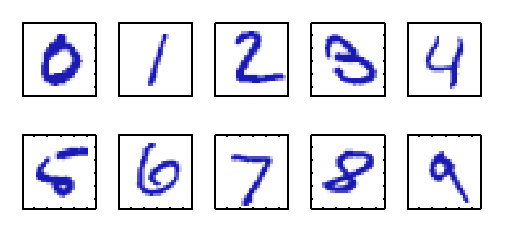
\includegraphics[width=8cm]{Figure1-1.eps}
	\caption{Examples of hand-written digits taken from US zip codes} 
	\label{fig:endb-flow} 
\end{figure}

	更优的结果是采用机器学习方法,这种方法中有一个很大的数字集合N $\{ \mathbf{x_1},$ $ \dots, \mathbf{x_N} \}$ 称为训练集,用来调整得到可适应模型的参数。在训练数据集中的数字分类已经提前给出,通常通过单独手工贴标签来检查他们。我们可以使用目标向量$\mathbf{t}$来表达一个数字的分类,表示对应数字的定义。对于用向量来表示的类别技术会在后面来进行讨论。注意到这里对于每一个数字图像$\mathbf{x}$,使用一个目标向量来表示。
	
	机器学习算法运行的结果可以表示为一个函数$\mathbf{y(x)}$,函数使用一个新的数字图像$\mathbf{x}$作为属兔,产生一个输出向量$\mathbf{y}$,其和目标向量的编码相同。函数$\mathbf{y(x)}$的精确格式在基于训练数据训练阶段时候确定,也被称作学习阶段。当模型确定后,就可以用来确定一个新的的数字图像,包括一个测试数据集。新样本的分类正确性不同于用来训练数据样本的能力称作一般化(generalization)。在实践应用中,
\section{图模型}


\chapter{The Second Chapter}
\section{密度估计}
密度是一个个嘎发哦发哦合法
\subsection{高斯密度}
\subsection{高斯密度}
\chapter{The First Chapter}
\section{daodaodaodoa}

\backmatter
% bibliography, glossary and index would go here.
\end{CJK}
\end{document}